\documentclass{article}
\usepackage{graphicx}
\usepackage{wrapfig}
\usepackage{amsmath}
\usepackage{subcaption}
\usepackage[margin=1.0in]{geometry}
\usepackage{lineno}
\usepackage{float}

\begin{document}
\section{Experiment}
Anion photoelectron spectroscopy (APES) measurements from 1996 indicate that the low-lying states of the CuO molecule are composed of 3d9 and 3d10 states [ref 48.pdf]. Shown below are the most recent APES measurements for the CuO molecule, all state assignments except for the $b^4\Sigma$ state have been verified by other experiments.

\begin{wrapfigure}{r}{0.4\textwidth}
  \begin{center}
    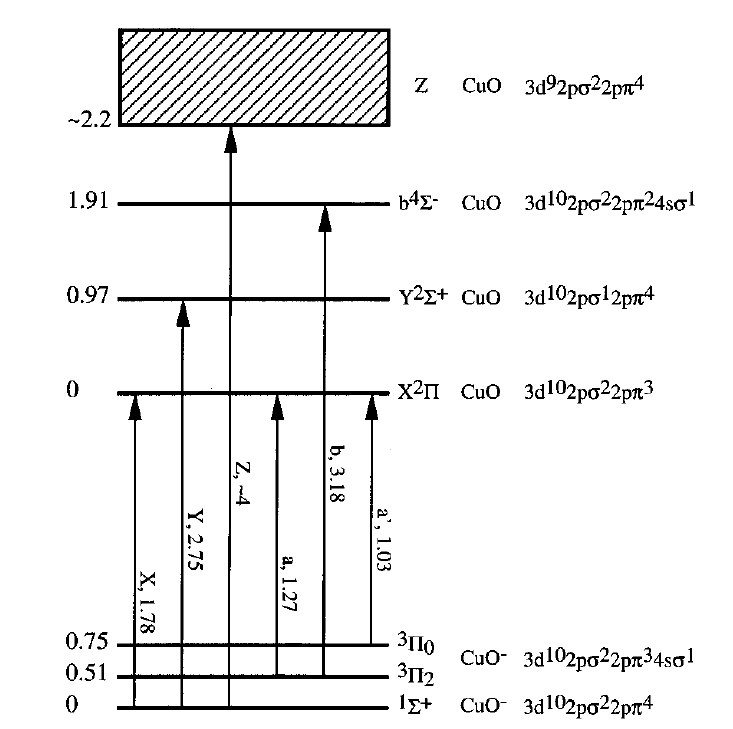
\includegraphics[width=0.3\textwidth]{APES.png}
  \end{center}
  \caption{APES measurements on CuO molecule.}
\end{wrapfigure}

The APES measurements yield a ground state of CuO is $X^2\Pi$ and the first excited state $Y^2\Sigma^+$, which are consistent with higher resolution PES measurements and various other theoretical and experimental measurements [multiple ref]. The $X^2\Pi \rightarrow Y^2\Sigma^+$ excitation corresponds to an excitation $O p_\sigma \rightarrow O p_\pi$, and has a measured energy of 0.97 eV. The APES measurements also find a block of excitations starting at 2.20 eV which correspond to the 3d9 excited states of CuO. Earlier measurements have found similar results. Further, both these APES measurements and Laser Induced Flourescence measurements in 1980 [ref] have found a quartet state at 1.91 eV. This state has been assigned as $^4\Sigma$, but the argumentation for its assignment is based on an assumption that the quartet state measured in APES is the lowest possible energy quartet state. 

Further, since the lowest energy states of the CuO molecule are 3d104s0, 3d94s0 and 3d94s1 in character, it is instructive to look at experimental measurements of the properties of the Cu$^+$ and Cu$^{2+}$ ions [ref]. The Cu$^{2+}$ ion has a ground state of character 3d94s0, and a first excited state around 6.7 eV of 3d84s1, indicating that the 3d8 sector of eigenstates may be ignored in our study. The Cu$^+$ ion has a ground state character of 3d10, and two excited states at 2.72 and 3.26 eV of character 3d94s1. These two low energy excited states differ in their total spin, the lower energy state being a $^3D$ state and the higher energy state being a $^1D$ state. This indicates to us that there is a Hund's coupling on the copper atom of $J_H = -0.54 eV$.

\section{Sampling scheme}
In order to do DMD we need to densely sample the low energy space (LES). In our case, we will define the LES as the span of a set of base states. Since we know that our system has a low energy 3d9 and 3d10 sector, we will consider base states with either 9 or 10 electrons in the d-orbitals. Further, in order to consider the effects of a possible Hund's coupling arising in our effective theory from the Cu atom $J_H$, we will need to consider states with both $S_z=1/2, 3/2$. When moving to QMC, we will not be able to consider linear combinations of states with different $S_z$, so in order to sample the effect of $J_H$ densely, we would also like to consider "spin-flip partner" states in the $S_z=1/2$ sector. Consider for example a state Cu3d9\! 4s1 O2p$_{\pi}$3 in the $S_z=1/2$ sector. The half-filled orbitals can have electrons with configuration $up\ up\ dn$ or $up\ dn\ up$, the prior which would have a Hund's descriptor $\frac{1}{2}$ and the latter $-\frac{1}{2}$. Further, we would like to use single determinant Slater-Jastrow wave functions since they have proven to be quite accurate trial wave functions on previous QMC calculations for transition metal oxide molecules [ref]. In order to meet all of these considerations, we chose to collect base states by using spin and spatial-symmetry targeted unrestricted Kohn Sham (UKS) [ref] single determinant states using a B3LYP functional [ref] and Trail-Needs basis with the corresponding pseudopotentials [ref]. Spin and spatial-symmetry targeted UKS cannot generate the following singly excited states: $(3d_\pi \rightarrow 2p_\pi)|GS\rangle, (3d_{z^2} \rightarrow 2p_\pi)|GS\rangle$. We tried and failed to converge these excited states using constrained DFT. Therefore the span of the basestates we are sampling is not the complete 3d9 and 3d10 sectors of the Hilbert space.

In order to sample the span of the base states we used a shell sampling technique which samples in shells of fixed radius around each of the base states using base state weights of 0.1 - 1.0 in increments of 0.1. Our final set of states in our span were then multiplied by a three-body Jastrow factor, which was optimized on the UKS ground state. Fixed node Diffusion Monte Carlo (FN-DMC) [ref] calculations were run with these states as trial wave functions with a timestep of 0.01 and Tmoves [ref]  in order to get 1-/2-density matrix elements and total energies.

\section{RDM basis}
There were two choices of the RDM basis that we could have used, either an IAO basis or an MO basis. The IAO basis is more theoretically pleasing because it's a set of functions which best capture the variation between the the Cu 3d, O 2p, and Cu 4s orbitals from our different base states. Further, the IAO basis is beneficial for representing local interactions since they are localized orbitals. However, the IAO basis has the drawback that many 1-body parameters will be correlated, for example $n_{p_\pi}$ and $t_\pi$. The MO basis choice is more arbitrary since we don't know a way of constructing "intrinsic molecular orbitals," but the RDM elements in this basis tend to vary in a less correlated fashion. This is because, to lowest order, excitations of CuO look very similar to single-particle molecular orbital excitations, so variations in the MO descriptor space are nearly orthogonal. In order to take advantage of the benefits of both bases, I chose to do my model fitting using a mixture of both bases: an MO basis for the non-interacting parts (n, t) and an IAO basis for the interacting pieces (J, U, etc.). In the end we can rotate the MO parameters into the IAO basis, leading to a fully localized representation of our model. The IAO basis I used was constructed on the collection of active MOs (Cu 3d, O 2p and Cu 4s) from every base state. The MO basis selected was the the set of active MOs from the first excited ROKS state of CuO. This is because the single-Slater determinant ground state of CuO from ROKS breaks O$p_x, p_y$ and Cu$d_{xz}, d_{yz}$ degeneracies. These degeneracies are restored in the first excited state ROKS calculation. Later in the analysis, a weighted linear regression (WLS) is used to fit our model, and it will be shown that the WLS assigns nearly zero weight to any sampled states which have a 1-rdm trace far less than 15, the total number of electrons expected in our active space, indicating that our MO model is functioning properly even though it was seemingly arbitrarily chosen. Ultimately, one just needs to ensure that the MO basis can capture variation in the electron number occupancy without having electrons vanish between relevant excitations.

\section{Model selection and fitting}
Model selection requires both an understanding of the CuO molecule's low energy excitations and some statistical analysis. We know that the lowest energy excitations of CuO are between the O p and Cu 4s orbitals, as these are the only excitations which allow for a 3d10 configuration. Further, given that we will be including 3d9 states, it's clear that we will need to at least consider the following non-interacting parameters:
$$\bar{\epsilon}_d, \bar{\epsilon}_z, \bar{\epsilon}_\pi, \bar{\epsilon}_s, \bar{t}_\pi, \bar{t}_{d_z^2 z}, \bar{t}_{4s z}, \bar{t}_{dz^2 4s}$$

Here the bars indicate parameters corresponding to RDM elements evaluated on our MO basis. In addition to these parameters, we know that the Cu$^+$ atom has a Hund's coupling, so we will consider a parameter $J_{sd}$ which is Hund's coupling between the Cu 4s and Cu 3d orbitals. Finally, some of our base states have a $4s^2$ occupation, and therefore including a $U_{4s}$ is necessary. Our final proposed model then looks like: 

$$ \boxed{\text{Proposed model: }\bar{\epsilon}_d, \bar{\epsilon}_z, \bar{\epsilon}_\pi, \bar{\epsilon}_s, \bar{t}_\pi, \bar{t}_{d_z^2 z}, \bar{t}_{4s z}, \bar{t}_{dz^2 4s}, J_{sd}, U_{4s}}$$

Since we know that $\bar{n}_d + \bar{n}_z + \bar{n}_\pi + \bar{n}_s = $ Const, we can eliminate $\bar{\epsilon}_d$ from our model since it is linearly dependent on the rest of the parameters. The left over occupation energies are certainly required in our model, given the knowledge we have of our low energy space. Since we know that $U_{4s}$ is required to describe the $4s^2$ states and that the $J_{sd}$ will probably play an important role as well, we just need to do model selection on the four hopping parameters. 

\subsection{Ordinary Linear Regression (OLS)}
To choose a model we first conduct OLS on all sixteen models which have subsets of these hopping parameters and conducting, We then removed from consideration any model which had OLS coefficients which were zero within two standard deviations of the mean, derived from boostrap resampling. We find that the $R^2$ scores between the resultant models are comparable and high, above 0.95. Since we were not able to sample the full low-energy (LE) space, the $R^2$ score itself is not a complete description of the validity of a model our LE space since an increased $R^2$ score can be due to overfitting of the model within our sample space (SS), leading to large extrapolation errors of our model predictions in the unsampled parts of the LE space. In order to investigate the extent of the extrapolation errors between models, we ran exact diagonalization (ED) calculations on our models in the IAO basis. After constructing the means and errors of the eigenvalues by bootstrapping, we removed any models with had an average error in the eigenvalues greater than 0.25 eV. This leaves just five models under consideration which have comparable $R^2$ score and small errors in the ED eigenvalues. Within these five models are two states which have a large extrapolation error as shown in the red boxes of Figure 2. The two states under consideration are a $(3dz^2 \rightarrow 2p_\pi)|GS\rangle, (2p_\pi \rightarrow 4s, d\bar{t}_\pi = 0)|GS\rangle$. As described earlier, the first state was not accessible by our sampling method and therefore no samples within SS can constrain the energy of this state. The latter state is also outside our sample set for a less obvious reason. Our sample space does contain a $(2p_\pi \rightarrow 4s)|GS\rangle$ state, however it has $d\bar{t}_\pi > 0$ because of the bonding nature of the $3d_\pi, 2p_\pi$ orbitals. In order to get the $d\bar{t}_\pi = 0$ state would require there to be no bonding between these orbitals or a linear combination with a state $d\bar{t}_\pi < 0$. Neither of these conditions are possible within our SS, hence the $(2p_\pi \rightarrow 4s, d\bar{t}_\pi = 0)|GS\rangle$ state is not contained in SS. Therefore, in order to pick one model out of our five potential models, we need to apply constraints on states which the ED may describe as low-energy, but which we did not sample.

%Figure 2
\begin{figure}[H]
\centering
\includegraphics[width=0.9\linewidth]{extrap.pdf}
\label{fig:extrap}
\caption{Two out of the five potential models with red boxes indicating the low-energy states which suffer a large extrapolation error.}
\end{figure}

\subsection{OLS with a prior}
In order to constrain samples outside of our set we can use information about eigenstates in LE - SS to construct a Bayesian prior. We know that LE - SS should be spanned by states of type $(3d_\pi \rightarrow 2p_\pi), (3d_{z^2} \rightarrow 2p_\pi), (3d_{z^2} \rightarrow 2s)$ and any composite excitations built on these states. While we cannot generate wave functions which represent these states using UKS, we can generate wave functions with higher energy which lack relevant orbital relaxations via molecular orbital excitations on the UKS ground state. Doing so and using these as trial functions in DMC, we find that all of these states have DMC energies $\geq$ 3.5 eV. This energy provides upper bounds for the lowest energy states with these certain occupation properties, and allows us to construct a pretty reasonable prior. 

$$\text{\textbf{Prior: }Any eigenstates outside of our SS should have an energy expectation } \langle H \rangle \sim \langle H_m \rangle \ge E_{cut} = 2 eV$$

The choice of 2eV as our lower bound for these eigenvalues was chosen because it falls significantly below 3.5 eV, allowing for the possibility of these states being heavily relaxed, but also constraining the energy to be higher than the lowest energy singly excited 3d10 states. In order to enforce this prior we use the following cost function to fit our linear models:

$$ \text{Cost} = \sum_i (y_i - \hat{y}_i)^2 + \lambda\sum_p Sig(E_{cut} - E_p), Sig(x) = \frac{1}{1+e^{-x}}.$$

The first term of this cost function is just the standard OLS cost with index $i$ running over our DMC samples within SS. The second term penalizes eigenstates which have energy below the chosen $E_{cut} = 2eV$. The index $p$ here runs over the eigenstates from section 4.1 which had a large extrapolation error. Therefore the second term is a simple implementation of our prior. The value of $\lambda$ can be varied in order to tradeoff the importance of each term. 

Starting with our five initial models, we allow $\lambda$ to vary between 0 to 40 with steps of 5 and conduct our linear regression with the above cost fuction. We then pass these models into ED and remove any models which have energy errors greater than 0.25 eV as before. Figure 3 shows the difference between $E_p$ and $E_{cut} = 2eV$ for the two different states composing the index $p$. It is pretty clear that the only model which is best at satisfying the prior for \textit{both} states is model 5. The regression with model 5 and $\lambda = 15$ match our prior the best and still have a good $R^2 = 0.96$ value and small noise. The final chosen model then accurately describes our SS and satisfies our prior for states within LE - SS and has form: 
\begin{multline}
 \boxed{\text{Final model }: \bar{\epsilon}_z = 0.65(7) eV, \bar{\epsilon}_\pi = 1.8(1) eV, \bar{\epsilon}_s = 3.0(1) eV, J_{sd} = -0.8(3) eV, U_{4s} = 3.8(5) eV}
\end{multline}

%Figure 3
\begin{figure}[H]
\centering
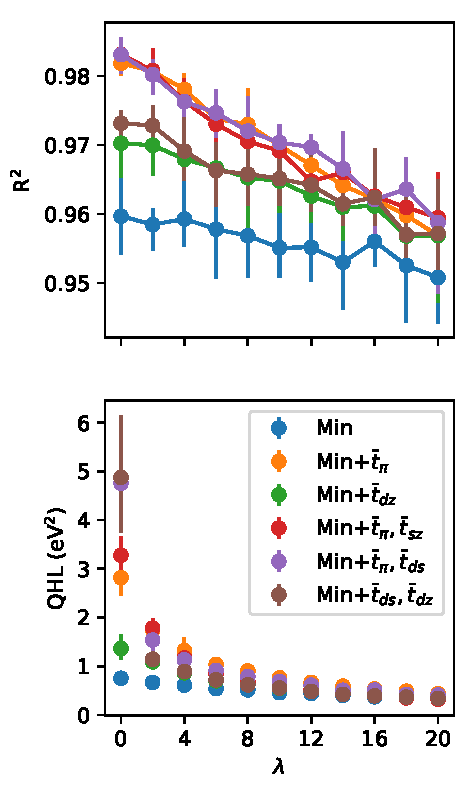
\includegraphics[width=0.9\linewidth]{prior.pdf}
\label{fig:extrap}
\caption{Difference from cutoff for different models for different $\lambda$.}
\end{figure}

\section{Comparison to DFT model}
We did an exact diagonalization on our Hamiltonian (2) using an FCI solver for a custom Hamiltonian in PySCF [ref]. Show in Figure 5 below are the lowest lying eigenstates of this model Hamiltonian and their single particle occupations. At $\beta=2$ (what we will be focusing on from here onwards) the ground state of our model matches that of experiment, namely it has an electron configuration of $Cu 3d^{10} O 2p_z^{1.75} O 2p_\pi^3 Cu 4s^{0.4}$, which would map to the approximate nominal filling of $Cu 3d^{10} O 2p_z^{2} O 2p_\pi^3 Cu 4s^{0}$, and is an $S_z=1/2$ state. The first excited state is an $S_z=1/2$ state at 1eV and which looks like an $O p_z \rightarrow O p_\pi$ excitation on the ground state, matching the results from APES. The first $3d^9$ state is also an $S_z=1/2$ state and sits at around 2.2 eV, which again matches the predictions of the APES measurements. Our model eigenstates therefore match very closely in the $S_z=1/2$ sector to the experimentally measured eigenstates in both energy and single particle properties.

There are also model eigenstates with $S_z=3/2$ which are low in energy. There is a quartet eigenstate at 2.0 eV which looks like an $O p_z \rightarrow Cu 4s$ excitation on the ground state, disagreeing with the experimental claims of a $^4\Sigma$ state at this energy. Our model predicts that the $^4\Sigma$ state is actually lower in energy at around 1.2 eV above the ground state, and looks like an $O p_\pi \rightarrow Cu 4s$ excitation on the ground state. These results indicate that a potential mislabelling may have occurred in experiment regarding the 2.0 eV quartet eigenstate, based on the faulty assumption that the lowest energy quartet state seen in the APES experiment was in fact the lowest energy quartet state. This may be due to the difficulty in measuring excitations to and out-of the $^4\Sigma$ state since it is so close in energy to the $S_z=1/2$ first excited state.

We can compare these results to those found from, for example, an ROKS or UKS calculation of the ground state for CuO. Typically one would take the ROKS/UKS eigenvalues to build an approximate non-interacting model of the system. Shown in Figure 6 are the ROKS/UKS eigenstates if we do so and exactly diagonalize in the $S_z=1/2,3/2$ sectors. The UKS eigenstates here are twice in number to the ROKS, since the UKS gives us two independent models, one for each spin channel. Studying just the ROKS model for now, we see that it does predict an eigenstate at 1 eV which resembles the $^2Y$ state, however there are no low energy $S_z=3/2$ states at all. All of the $S_z=3/2$ states are $>$ 3eV above the ground state. I believe this is due, in part, to the lack of relaxation effects present in the 1-particle model, as the orbitals of excited states of the CuO molecule are augmented relative to the orbitals of the ground state. Further, the exclusion of the $J_{sd}$ pushes the $S_z=3/2$ states higher in energy than expected in reality. The UKS model also fails to describe the $S_z=3/2$ states accurately for similar reasons.


\end{document}